\documentclass[11pt,letterpaper,titlepage]{article}
\usepackage{fancyhdr}
\usepackage[left=0.75in, right=0.75in, bottom=1.0in]{geometry}
\usepackage{lastpage}
\usepackage{titleref}
\usepackage{booktabs}
\usepackage{appendix}
\appendixtitleon
\appendixtitletocon

\makeatletter

%================== List of figures and tables mods
\usepackage{tocloft}
\usepackage[labelfont=bf]{caption}

\renewcommand{\cftfigpresnum}{Figure\ }
\renewcommand{\cfttabpresnum}{Table\ }

\newlength{\mylenf}
\settowidth{\mylenf}{\cftfigpresnum}
\setlength{\cftfignumwidth}{\dimexpr\mylenf+1.5em}
\setlength{\cfttabnumwidth}{\dimexpr\mylenf+1.5em}


\newcommand{\half}{\frac{1}{2}}


%=================== Graphics
\usepackage{graphicx}
\usepackage[breakwords]{truncate}
\usepackage{float}
\usepackage{array}
\usepackage{amsmath}
\usepackage{mdframed}
\usepackage{fancyvrb}
\usepackage{float}
\usepackage{cancel}
\usepackage{amssymb}
\graphicspath{ {images/} }
\usepackage[usenames,dvipsnames,svgnames,table]{xcolor}
\usepackage[defaultlines=2,all]{nowidow}
\usepackage{listings}
\usepackage{color}
\definecolor{Brown}{cmyk}{0,0.81,1,0.60}
\definecolor{OliveGreen}{cmyk}{0.64,0,0.95,0.40}
\definecolor{CadetBlue}{cmyk}{0.62,0.57,0.23,0}
\usepackage{pdflscape}
\usepackage{relsize}
\usepackage{verbatim}
\usepackage{tabto}


%=================== Settings
\renewcommand{\baselinestretch}{1.2}
\definecolor{gray}{rgb}{0.4 0.4 0.4}
\newcommand{\stimes}{{\times}}

\begin{document}
\newcommand{\NSCDOCNUMBR}{NSC-REP-15-X}         %Put document number here
\newcommand{\NSCDOCSUBJT}{TECHNICAL REPORT: }   %Put document subject here
\newcommand{\NSCDOCTITLE}{$THERMOFLOW$ - System level Thermal-Hydraulics in $ChiTech$}       %Put document title here
\newcommand{\NSCDOCDATE} {March, 2016}    %Put document date here
\newcommand{\NSCDOCREV}  {Rev 1.01} %Put revision number here

\lstset{language=C++,frame=ltrb,framesep=4pt,basicstyle=\linespread{0.8} \small,
	keywordstyle=\ttfamily\color{OliveGreen},
	identifierstyle=\ttfamily\color{CadetBlue}\bfseries,
	commentstyle=\color{Brown},
	stringstyle=\ttfamily,
	showstringspaces=ture }


%################################# TITLE PAGE ########################
\begin{titlepage}
	\pagestyle{fancy}
	\vspace*{1.0cm}
	\centering
	%\includegraphics{NSC_Logo} \par
	\vspace{1cm}
	%\centering
	%{\Large\bfseries  \NSCDOCNUMBR   \par}
	\vspace{.25cm}
	%\centering
	{\Large\bfseries  \NSCDOCSUBJT \par} 
	{\Large\bfseries \NSCDOCTITLE  \par}
	\vspace{1cm}
	{\Large \NSCDOCDATE \par}
	\vspace{1.0cm}
	{\Large Jan Vermaak \& Guillermo Villanueva \par}
	{\Large \NSCDOCREV \par}
		
	\begin{comment}
	\renewcommand{\arraystretch}{2.0}
	\begin{tabular}{| m{2.5cm} | m{4.5cm} | m{4.5cm} |}
		\cline{2-3}
		\multicolumn{1}{c|}{} & \bfseries{Name} & \bfseries{Signature \& Date} \\ \hline
		\bfseries{Prepared} &     &     \\ \hline
		\bfseries{Reviewed} &     &     \\ \hline
		\bfseries{Reviewed} &     &     \\ \hline
	    \bfseries{Approved} &     &     \\ \hline
	\end{tabular} \par
	\end{comment}
	\begin{center}
		\begin{minipage}[c]{0.45\textwidth}
			\begin{figure}[H]
			
				
\includegraphics[width=3in]{Logo2_Medium.png}
			\end{figure}
		\end{minipage}
	\end{center}
	\vspace{2cm}
	%NSC-FRM-15-1 Rev.1
\end{titlepage}


\pagestyle{fancy}
\rfoot{Page \thepage \ of \pageref{LastPage}}
%\cfoot{NSC-FRM-15-1 Rev.1}
\cfoot{}
\lfoot{\truncate{14cm}{\NSCDOCTITLE}}
\rhead{}
\chead{\currentname}
\lhead{}
\renewcommand{\footrulewidth}{0.4pt}
\tableofcontents
\addtocontents{toc}{~\hfill\textbf{Page}\par}

\listoffigures
\listoftables
\chead{Contents}


\newpage
\chead{1 Conservation equations}
\section{Conservation equations}
The overall objective is that we want to solve the following four field variables:
\begin{itemize}
\item Pressure, $P$
\item Internal energy, $u$
\item Velocity, $v$
\item Density, $\rho$
\end{itemize}

\vspace{0.25cm}
\noindent
In order to do this we apply the conservation equations to the volume shown in Figure \ref{figure:ZZZ_ControlVolume} below:
	\begin{center}
		\begin{minipage}[c]{0.7\textwidth}
	
			\begin{figure}[H]
			
				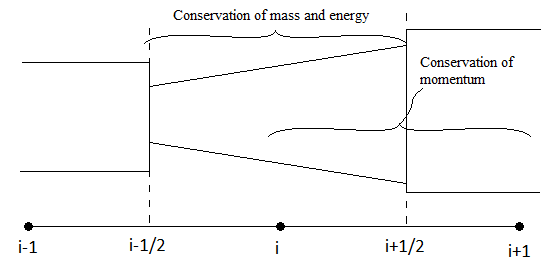
\includegraphics[width=5in]{ZZZ_ControlVolume.png}
				\caption{Simple layout of control volumes.}
				\label{figure:ZZZ_ControlVolume}
			\end{figure}
		\end{minipage}
	\end{center}
\vspace{0.5cm}

\newpage
\subsection{Conservation of Mass}
Even though we will be dealing with incompressible liquids, the liquids can exist at different temperatures and therefore different densities, $\rho$. The conservation of mass requires as a function of time, $t$:

\begin{equation*}
\frac{d\rho}{dt}=\frac{1}{V}\int_S \rho.(\vec{v}\cdot \hat{n}).dA
\end{equation*}
\newline
\noindent And by applying it to the control volume:

\begin{equation}
\frac{d\rho_i}{dt} = \frac{1}{V_i}\biggr[ (\rho.A.v)_{i-\half}-(\rho.A.v)_{i+\half} \biggr]
\end{equation}

\noindent 
Where: 
\newline \noindent $v$ \quad = velocity.
\newline \noindent $V$ \quad = Volume.
\newline \noindent $A$ \quad = Area.
\newline \noindent $\hat{n}$ \quad = Surface normal.

\subsection{Conservation of Momentum}
The change in momentum, $m_i.v_{i}$, in a control volume must balance the momentum of all the in and out flows as well as any forces applied:

\begin{equation*}
\frac{d(mv)_i}{dt}=\int_S \rho. |v|. (\vec{(v)}\cdot \hat{n}).dA + \int_S P.\hat{n}.dA+mg-F_{friction}
\end{equation*}
\newline
\noindent For a control volume as shown in Figure \ref{figure:ZZZ_ControlVolume} we have:

\begin{equation*}
\begin{aligned}
\frac{d(\rho v)_i}{dt}&=\frac{1}{V_i} \biggr[ (\rho A v^2 d)_{i-\half} +(\rho A v^2 d)_{i+\half}  \biggr] \\
&+\frac{1}{V_i} \biggr[ (PA)_{i-\half} - (PA)_{i+\half} \biggr]+\rho_ig_i-\frac{1}{V_i} F_{\tau}
\end{aligned}
\end{equation*}
\newline
Where $d$ is the direction value (either $+1$ or $-1$), $F_{\tau}$ is the wall friction force and $g_i$ is the gravitational component (i.e. $g_i=g.sin\theta_i$, $g=-9.81 m.s^{-2}$). In later derivations of the numerical representation it is more convenient to define the conservation of momentum equation about a boundary by:

\begin{equation*}
\frac{d(\rho v)}{dt}=-\rho \frac{d(v^2)}{dx} -\frac{dP}{dx}+\rho g - \frac{\tau}{L}
\end{equation*}
\newline
Applied to the boundary junction, $i+\half$, we can write:
\begin{equation}
\begin{aligned}
\frac{d(\rho v)_{i+\half}}{dt}=&-\frac{\rho_{i+\half}}{2}\cdot\frac{d_i.(v_{i})^2+d_{i+1}.(v_{i+1})^2}{\Delta x_{i+\half}} \\
&-\frac{P_{i+1}-P_i}{\Delta x_{i+\half}} + \rho_{i+\half}.g_{i+\half}-\frac{F_{\tau,i}}{2V_i}-\frac{F_{\tau,i+1}}{2V_{i+1}} \\
&+\frac{\rho_{i+\half}}{2}\cdot VISC_{i+\half}
\end{aligned}
\end{equation}
\newline
Where $VISC_{i+\half}$ is an artificial viscosity term needed to correct for different junction velocities:
\begin{equation*}
VISC_{i+\half}=|v_{i+1}|\biggr[ v_{i+\frac{3}{2}} \biggr(\frac{A_{i+\frac{3}{2}}}{A_{i+\half}} \biggr) - v_{i+\half}       \biggr] - 
|v_{i}|\biggr[ v_{i+\half}  - v_{i-\half} \biggr(\frac{A_{i-\half}}{A_{i+\half}} \biggr)      \biggr]
\end{equation*}
\noindent 
Also, $\Delta x_{i+\half}$ is the distance between control volumes $i$ and $i+1$, $g_{i+\half}$ is the gravitational force component (function of inclination angle between control volume centroids). The wall friction force can be calculated from the Darcy Friction Factor, $f$:

\begin{equation*}
F_{\tau}=\half f \rho \frac{L}{D_H} A v^2
\end{equation*} 
\noindent Therefore:

\begin{equation*}
\begin{aligned}
F_{\tau,i}&=\frac{1}{4} f_i \rho_i \frac{L_i}{D_{H,i}}A_i v_i^2 \\
F_{\tau,i+1}&=\frac{1}{4} f_{i+1} \rho_{i+1} \frac{L_{i+1}}{D_{H,i+1}}A_{i+1} v_{i+1}^2 \\
\end{aligned}
\end{equation*}
\newline
\noindent
In these equations $L_i$ and $D_{H,i}$ are the length and hydraulic diameter of the $i$-th control volume.


\newpage
\subsection{Conservation of Energy}
The total energy of the system, $E$, must balance that of the in and out flow including the work performed and the heat transfer into the system:

\begin{equation*}
\frac{dE}{dt}=\int_S \rho.(\vec{v}\cdot \hat{n}).e.dA + Q - W -E_{loss}
\end{equation*}

\noindent 
Where: 
\newline \noindent $e$ \quad = Specific energy of the system.
\newline \noindent $Q$ \quad = Heat transfer into the system.
\newline \noindent $W$ \quad = Work leaving the system.
\newline \noindent $E_{loss}$ \quad = Dissipative energy losses.
\newline
\newline
The components of energy are internal energy, $U$, kinetic energy, $\half mv^2$, and potential energy, $mgz$:

\begin{equation*}
E= m.e = m.(u+\half v^2+gz)
\end{equation*}
\newline
For most control volume fluid flows where the control volume flow rate is small compared to its area it is often acceptable to neglect the kinetic energy term. Also, since it undergoes no change in elevation we can neglect the elevation change (but only for the control volume, not the junctions).
\newline
\newline
The heat transfer into the system is normally associated with some heat flux, $\dot{q}$, and the total heat transfer surface, $A_s$, therefore:

\begin{equation*}
Q_i=\dot{q}_i.A_{s,i}
\end{equation*}
\newline
The components of work include shaft work, $W_{shaft}$, and pressure work, $W_{pressure}$. For this case we will consider only pressure work:

\begin{equation*}
W_{pressure}=(P.A.v)_{i+\half} - (P.A.v)_{i-\half} 
\end{equation*}
\newline
\noindent
From here the energy conservation equation becomes:

\begin{equation*}
\begin{aligned}
\frac{d}{dt} \biggr( m.u \biggr)&=(\rho Av)_{i-\half}.(u+gz)_{i-\half} - (\rho Av)_{i+\half}.(u+gz)_{i+\half} \\
&+\dot{q}_i.A_{s,i} + \biggr[   (P.A.v)_{i-\half} - (P.A.v)_{i+\half}   \biggr] + E_{loss}
\end{aligned}
\end{equation*}
\newline
\noindent
Dividing by the volume we get:

\begin{equation}
\begin{aligned}
\frac{d(\rho.u)_i}{dt} &=\frac{1}{V_i}\biggr[ (\rho Av)_{i-\half}.(u+gz)_{i-\half} - (\rho Av)_{i+\half}.(u+gz)_{i+\half} \biggr] \\
&+\frac{A_{s,i}}{V_i}\dot{q}_i + \frac{1}{V_i}\biggr[   (P.A.v)_{i-\half} - (P.A.v)_{i+\half}   \biggr] + \frac{1}{V_i}\biggr[  E_{loss,i-\half} +E_{loss,i+\half}   \biggr]
\end{aligned}
\end{equation}
\newline
\noindent The energy loss term includes both dynamic losses at the junctions and those within the control volume, however, for simplicity we will only consider the loss associated with junction losses for which the pressure loss is given by:

\begin{equation*}
\Delta P = \half K \rho  v^2
\end{equation*}
\newline
\noindent Where $K$ is a dimensionless parameter dependent on the geometry. The energy loss associated with this factor is:

\begin{equation*}
E_{loss,i-\half}=
\begin{cases}
(\Delta P.A.v)_{i-\half} = \half  K_{i-\half} (\rho A v^3)_{i-\half}     &,v_{i-\half}>0 \\
0    &,v_{i-\half}<0
\end{cases}
\end{equation*}
\newline
\noindent Similarly:
\begin{equation*}
E_{loss,i+\half}=
\begin{cases}
(\Delta P.A.v)_{i+\half} = \half  K_{i+\half} (\rho A v^3)_{i+\half}     &,v_{i+\half}<0 \\
0    &,v_{i+\half}>0
\end{cases}
\end{equation*}


\subsection{Equation of state}
In addition to the conservation equations, there is the equation of state. For the incompressible liquids of this simulation we can approximate the equation of state as:

\begin{equation}
\begin{aligned}
u&=-0.002053148 \ \rho^3+5.927524805 \ \rho^2-5710.176493 \ \rho+1835863.516 \\
\rho&=7.88656E-06 \ T^3-0.004477273 \ T^2-0.059652292 \ T+1001.25303\\
\mu&=1.66762E-08 \ \rho^3-4.83243E-05 \ \rho^2+0.046680223 \ \rho-15.03102921\\
\end{aligned}
\end{equation}






\newpage
\chead{2 Numerical solution}
\section{Numerical solution}
The conservation of momentum equations conveniently couples the pressure field and velocities and therefore is used implicitly to determine the pressures at time $n+1$.

\subsection{Conservation of Mass - finite difference formulation}
The finite difference formulation is as follows:


\begin{equation}
\frac{\rho_i^{n+1} - \rho_i^{n}}{\Delta t} = \frac{1}{V_i}\biggr[ (\rho.A)_{i-\half}^{n}v_{i-\half}^{n+1}-(\rho.A)_{i+\half}^{n} v_{i+\half}^{n+1} \biggr]
\end{equation}




\subsection{Conservation of Momentum - finite difference formulation}
Because no other future time equation has pressure as a variable we opt to include pressure at time $n+1$ as an implicit variable. We manipulate the original conservation of mass equation for junction $i+\half$:
\begin{equation*}
\begin{aligned}
\frac{d(\rho v)_{i+\half}}{dt}=&-\frac{\rho_{i+\half}}{2}\cdot\frac{d_i.(v_{i})^2+d_{i+1}.(v_{i+1})^2}{\Delta x_{i+\half}} \\
&-\frac{P_{i+1}-P_i}{\Delta x_{i+\half}} + \rho_{i+\half}.g_{i+\half}-\frac{F_{\tau,i}}{2V_i}-\frac{F_{\tau,i+1}}{2V_{i+1}} \\
&+\frac{\rho_{i+\half}}{2}\cdot VISC_{i+\half}
\end{aligned}
\end{equation*}

\noindent We use the following time notation:

\begin{equation}
\begin{aligned}
\frac{\rho_{i+\half}^{n}.v_{i+\half}^{n+1}-\rho_{i+\half}^n.v_{i+\half}^n}{\Delta t} =&- \rho_{i+\half}^n\cdot\frac{d_i.(v_{i}^n)^2-d_{i+1}.(v_{i+1}^n)^2}{\Delta x_{i+\half}}     \\
&-\frac{P_{i+1}^{n+1}-P_i^{n+1}}{\Delta x_{i+\half}} +\rho_{i+\half}^n.g_{i+\half} \\
&-\frac{1}{2V_i}F_{\tau,i}^n- \frac{1}{2V_{i+1}}F_{\tau,i+1}^n + \rho_{i+\half}^n\cdot\frac{VISC_{i+\half}^n}{\Delta x_{i+\half}}
\end{aligned}
\end{equation}
\newline
Where:
\begin{equation*}
VISC_{i+\half}^n=|v_{i+1}^n|\biggr[ v_{i+\frac{3}{2}}^n \biggr(\frac{A_{i+\frac{3}{2}}}{A_{i+\half}} \biggr) - v_{i+\half}^n       \biggr] - 
|v_{i}^n|\biggr[ v_{i+\half}^n  - v_{i-\half}^n \biggr(\frac{A_{i-\half}}{A_{i+\half}} \biggr)      \biggr]
\end{equation*}
\newline
\noindent In the equations above we included implicit time instances to pressure in order to semi-implicitly couple the system.
\newline
\newline
We can find the same equation for junction $i-\half$:
\begin{equation}
\begin{aligned}
\frac{\rho_{i-\half}^{n}.v_{i-\half}^{n+1}-\rho_{i-\half}^n.v_{i-\half}^n}{\Delta t} =&- \rho_{i-\half}^n\cdot\frac{d_{i-1}.(v_{i-1}^n)^2+d_{i}.(v_{i}^n)^2}{\Delta x_{i-\half}}     \\
&-\frac{P_{i}^{n+1}-P_{i-1}^{n+1}}{\Delta x_{i-\half}} +\rho_{i-\half}^n.g_{i-\half} \\
&-\frac{1}{2V_{i-1}}F_{\tau,i-1}^n- \frac{1}{2V_{i}}F_{\tau,i}^n
+ \rho_{i-\half}^n\cdot\frac{VISC_{i-\half}^n}{\Delta x_{i-\half}}
\end{aligned}
\end{equation}
\newline
Where:
\begin{equation*}
VISC_{i-\half}^n=|v_{i}^n|\biggr[ v_{i+\frac{1}{2}}^n \biggr(\frac{A_{i+\frac{1}{2}}}{A_{i-\half}} \biggr) - v_{i-\half}^n       \biggr] - 
|v_{i-1}^n|\biggr[ v_{i-\half}^n  - v_{i-\frac{3}{2}}^n \biggr(\frac{A_{i-\frac{3}{2}}}{A_{i-\half}} \biggr)      \biggr]
\end{equation*}


\vspace{1cm}
\subsection{Conservation of Energy - finite difference formulation}
We start with the original conservation of energy equation:

\begin{equation*}
\begin{aligned}
\frac{d(\rho.u)_i}{dt} &=\frac{1}{V_i}\biggr[ (\rho Av)_{i-\half}.(u+gz)_{i-\half} - (\rho Av)_{i+\half}.(u+gz)_{i+\half} \biggr] \\
&+\frac{A_{s,i}}{V_i}\dot{q}_i + \frac{1}{V_i}\biggr[   (P.A.v)_{i-\half} - (P.A.v)_{i+\half}   \biggr] + \frac{1}{V_i}\biggr[  E_{loss,i-\half} +E_{loss,i+\half}   \biggr]
\end{aligned}
\end{equation*}
\newline
\noindent We now discretize the left side and set the right side to correspond to time $n$.

\begin{equation}
\begin{aligned}
\frac{(\rho_i^{n+1}.u_i^{n+1}-  \rho_i^{n}.u_i^{n})}{\Delta t}&=\frac{1}{V_i}\biggr[ (\rho Au)_{i-\half}^n.v_{i-\half}^{n+1} -(\rho Au)_{i+\half}^n.v_{i+\half}^{n+1} \biggr] \\
&+\frac{1}{V_i}\biggr[ (\rho Agz)_{i-\half}^n.v_{i-\half}^{n+1} -(\rho Agz)_{i+\half}^n.v_{i+\half}^{n+1} \biggr] \\
&+\frac{A_{s,i}}{V_i}\dot{q}_i^n + \frac{1}{V_i}\biggr[   (P.A)_{i-\half}^n.v_{i-\half}^{n+1} - (P.A)_{i+\half}^n.v_{i+\half}^{n+1}   \biggr] \\
&+ \frac{1}{V_i}E_{loss}^n
\end{aligned}
\end{equation}



\subsection{Equation of state numerical implementation}
In order to implement a linear approximation to the equation of state we linearize the Equation of State by determine the derivative at the old time values. Specifically this applies to the relation of internal energy, $u$, to the density, $\rho$:

\begin{equation*}
\begin{aligned}
\frac{d(u_i^{n+1})}{d\rho}&=\frac{d}{d\rho} \biggr[  -0.002053148 \ \rho^3+5.927524805 \ \rho^2-5710.176493 \ \rho+1835863.516    \biggr] \\
                          &=-0.006159444 \ (\rho_{i}^{n})^2+11.85504961 \ (\rho_{i}^{n}) -5710.176493 
\end{aligned}
\end{equation*}
\newline
From this derivative we find the linearized equation of state:

\begin{equation}
u_{i}^{n+1} = \frac{d(u_i^{n+1})}{d\rho}\cdot \rho_{i}^{n+1} -\frac{d(u_i^{n+1})}{d\rho}\cdot\rho_{i}^{n} +  u_{i}^{n}   
\end{equation}






\newpage
\subsection{Unknowns in the available equations}
The "new" time values that require solving are found in the following terms:

\begin{equation*}
\begin{aligned}
&\rho_i^{n+1}, v_{i+\half}^{n+1}, v_{i-\half}^{n+1}, \ from \ equation \ 5 \\
&v_{i+\half}^{n+1}, P_{i+1}^{n+1},P_{i}^{n+1}, \ from \ equation \ 6 \\
&v_{i-\half}^{n+1}, P_{i-1}^{n+1},P_{i}^{n+1}, \ from \ equation \ 7 \\
&\rho_i^{n+1}, u_{i}^{n+1}, v_{i-\half}^{n+1},v_{i+\half}^{n+1}, \ from \ equation \ 8 \\
&\rho_i^{n+1}, u_{i}^{n+1}, \ from \ equation \ 9
\end{aligned}
\end{equation*}
\newline
However, the some unknowns in the old time variables also exist. we change $\rho_{i+\half}^{n}$ according to:

\begin{equation*}
\rho_{i+\half}^{n}=
\begin{cases}
\rho_{i}^{n}       &, v_{i+\half}^n\ge 0 \\
\rho_{i+1}^{n}     &, v_{i+\half}^n<0
\end{cases}
\end{equation*}
\newline
We then compute $v_i^{n}$ from the arithmetic average of the junction velocities according to:

\begin{equation*}
v_i^{n}=v_{i-\half}^n \frac{A_{i-\half}}{2A_i} + v_{i+\half}^n \frac{A_{i+\half}}{2A_i}
\end{equation*}
\newline
With this velocity known we can calculate the dimensionless Reynold's number, $Re$:

\begin{equation*}
Re_i=\frac{\rho_i^n v_n^n D_{H,i}}{\mu_i^n}
\end{equation*}
\newline
The Reynold's number features in the calculation of the Darcy friction factor, $f$, which is contained in a different formula depending on the flow regime, i.e. the laminar flow regime at $Re<2300$ and the turbulent flow regime at $Re>4000$. In the laminar regime the factor is calculated from:

\begin{equation*}
f=\frac{64}{Re}
\end{equation*}
\newline
In the turbulent regime the factor can be calculated from the Colebrook-White equation:

\begin{equation*}
\frac{1}{\sqrt{f}}=-2\textrm{log}\biggr( \frac{\epsilon}{3.7D_H}  + \frac{2.51}{Re \sqrt{f}}   \biggr)
\end{equation*}
\newline
This equation is a transcendental equation (i.e. no analytical solution), however, lookup tables can be generated as a function of $Re$ for a given roughness $\epsilon$ using a Newton-Raphson numerical scheme. This lookup table generator needs to accommodate the transition between the laminar flow regime at $Re<2300$ and the turbulent flow regime at $Re>4000$. One such method is to calculate a spline fit between the two regimes. An example of such a generator is shown below.




\subsection{Semi-implicit approach}
From equation 5 we can solve for $\rho_i^{n+1}$ and from equation 4 we can solve for $u_i^{n+1}$. From equation 7 we can solve for $v_{i+\half}^{n+1}$. Now the only variables left unsolved is the pressures $P_{i+1}^{n+1}$ and $P_{i}^{n+1}$.
\newline
\newline
Hence we are left with the conservation of momentum equation with the unknowns $P_{i}$ and $P_{i+1}$. Therefore, in a single time step where we have $I$ amount of control volumes as shown in Figure \ref{figure:ZZZ_SimpleSystem} below, we will have $I$ unknowns and $I$ amount of momentum equations. 

	\begin{center}
		\begin{minipage}[c]{0.85\textwidth}
	
			\begin{figure}[H]
			
				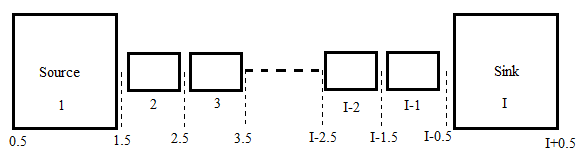
\includegraphics[width=6in]{ZZZ_SimpleSystem.png}
				\caption{Simple layout of multiple control volumes.}
				\label{figure:ZZZ_SimpleSystem}
			\end{figure}
		\end{minipage}
	\end{center}
\vspace{0.5cm}










\newpage
\subsection{Solution algorithm}

\textbf{Step 1}\newline
Load all control volumes. Input parameters:
\begin{itemize}
\item Area, $A$
\item Length, $L$
\item Pressure, $P$
\item Temperature, $T$
\item Elevation change, $\Delta z$
\item Wall roughness, $\epsilon$
\item Hydraulic diameter, $D_H$
\item Surface area, $A_s$
\end{itemize}



\vspace{0.5cm}\noindent
\textbf{Step 2}\newline
Load all junctions. Input parameters:
\begin{itemize}
\item Junction velocity, $v$
\item Area, $A$
\item Loss factor, $K$
\end{itemize}






\vspace{0.5cm}\noindent
\textbf{Step 3}\newline
\noindent Determine density, $\rho_i$, from:

\begin{equation*}
\rho=7.88656E-06 \ T^3-0.004477273 \ T^2-0.059652292 \ T+1001.25303
\end{equation*}
\newline
Internal energy, $u_i$, from:
\begin{equation*}
u=-0.002053148 \ \rho^3+5.927524805 \ \rho^2-5710.176493 \ \rho+1835863.516 
\end{equation*}
\newline
Dynamic viscosity, $\mu_i$, from:
\begin{equation*}
\mu=1.66762E-08 \ \rho^3-4.83243E-05 \ \rho^2+0.046680223 \ \rho-15.03102921
\end{equation*}
\newline
Velocity, $v_i$, from:
\begin{equation*}
v_i=v_{i-\half}\frac{A_{i-\half}}{2A_i} + v_{i+\half} \frac{A_{i+\half}}{2A_i}
\end{equation*}



\vspace{0.5cm}\noindent
\textbf{Step 4}\newline
Determine all junction and control volume $z$ values using control volume $\Delta z$ values.




\vspace{0.5cm}\noindent
\textbf{Step 5 - Repeat from for new time steps}\newline
Determine $\rho_{i-\half}^n$ and $\rho_{i+\half}^n$ as follows:
\begin{equation*}
\rho_{i-\half}^n=
\begin{cases}
\rho_{i-1}^n     &,v_{i-\half}\ge 0 \\
\rho_{i}^n    &,v_{i-\half}<0
\end{cases}
\end{equation*}
\begin{equation*}
\rho_{i+\half}^n=
\begin{cases}
\rho_{i}^n     &,v_{i+\half}\ge 0 \\
\rho_{i+1}^n    &,v_{i+\half}<0
\end{cases}
\end{equation*}
And similarly for $u_{i-\half}^n$ and $u_{i+\half}$ from:
\begin{equation*}
u_{i-\half}^n=
\begin{cases}
u_{i-1}^n     &,v_{i-\half}>0 \\
u_{i}^n    &,v_{i-\half}<0
\end{cases}
\end{equation*}
\begin{equation*}
u_{i+\half}^n=
\begin{cases}
u_{i}^n     &,v_{i+\half}>0 \\
u_{i+1}^n    &,v_{i+\half}<0
\end{cases}
\end{equation*}



\vspace{0.5cm}\noindent
\textbf{Step 6}\newline
Calculate control volume quantities. First, velocity, $v_i$, from:
\begin{equation*}
v_i=v_{i-\half}\frac{A_{i-\half}}{2A_i} + v_{i+\half} \frac{A_{i+\half}}{2A_i}
\end{equation*}
Dynamic viscosity, $\mu_i$, from:
\begin{equation*}
\mu=1.66762E-08 \ \rho^3-4.83243E-05 \ \rho^2+0.046680223 \ \rho-15.03102921
\end{equation*}
Reynolds number, $Re_i$, from:
\begin{equation*}
Re_i=\frac{\rho_i^n v_n^n D_{H,i}}{\mu_i^n}
\end{equation*}
Drag force, $F_{\tau}$, from:
\begin{equation*}
F_{\tau,i}=\frac{1}{4} f_i \rho_i \frac{L_i}{D_{H,i}}A_i v_i^2 
\end{equation*}
Junction pressure drop losses, $E_{loss}$, from:
\begin{equation*}
E_{loss,i-\half}=
\begin{cases}
(\Delta P.A.v)_{i-\half} = \half  K_{i-\half} (\rho A v^3)_{i-\half}     &,v_{i-\half}>0 \\
0    &,v_{i-\half}<0
\end{cases}
\end{equation*}
\newline
\noindent Similarly:
\begin{equation*}
E_{loss,i+\half}=
\begin{cases}
(\Delta P.A.v)_{i+\half} = \half  K_{i+\half} (\rho A v^3)_{i+\half}     &,v_{i+\half}<0 \\
0    &,v_{i+\half}>0
\end{cases}
\end{equation*}


\vspace{0.5cm}\noindent
\textbf{Step 7}\newline
Determine the elements of equation 5:
\begin{equation*}
\frac{\rho_i^{n+1} - \rho_i^{n}}{\Delta t} = \frac{1}{V_i}\biggr[ (\rho.A)_{i-\half}^{n}v_{i-\half}^{n+1}-(\rho.A)_{i+\half}^{n} v_{i+\half}^{n+1} \biggr]
\end{equation*}
\newline
Where the elements are:
\begin{equation*}
\begin{aligned}
B_5&=\frac{\Delta t (\rho.A)_{i-\half}^{n}}{V_i}\\
C_5&=\frac{\Delta t (\rho.A)_{i+\half}^{n}}{V_i}
\end{aligned}
\end{equation*}
\newline
To get:
\begin{equation}
\begin{aligned}
\rho_i^{n+1}&=\rho_i^{n}+B_5.v_{i-\half}^{n+1} - C_5.v_{i+\half}^{n+1}\\
\end{aligned}
\end{equation}




\newpage \noindent
\textbf{Step 8}\newline
Determine the elements of equation 6:
\begin{equation*}
\begin{aligned}
\frac{\rho_{i+\half}^{n}.v_{i+\half}^{n+1}-\rho_{i+\half}^n.v_{i+\half}^n}{\Delta t} =&- \rho_{i+\half}^n\cdot\frac{d_i.(v_{i}^n)^2-d_{i+1}.(v_{i+1}^n)^2}{\Delta x_{i+\half}}     \\
&-\frac{P_{i+1}^{n+1}-P_i^{n+1}}{\Delta x_{i+\half}} +\rho_{i+\half}^n.g_{i+\half} \\
&-\frac{1}{2V_i}F_{\tau,i}^n- \frac{1}{2V_{i+1}}F_{\tau,i+1}^n
\end{aligned}
\end{equation*}
\newline
Where the elements are:
\begin{equation*}
\begin{aligned}
B_6&=\rho_{i+\half}^n.v_{i+\half}^n\\
C_6&=\Delta t\rho_{i+\half}^n\cdot\frac{d_i.(v_{i}^n)^2-d_{i+1}.(v_{i+1}^n)^2}{\Delta x_{i+\half}}\\
D_6&=\frac{\Delta t}{\Delta x_{i+\half}}, \quad E_6=\Delta t \rho_{i+\half}^n.g_{i+\half} \\
F_6&=\frac{\Delta t}{2V_i}F_{\tau,i}^n, \quad G_6=\frac{\Delta t}{2V_{i+1}}F_{\tau,i+1}^n \\
H_6&=\frac{B_6-C_6+E_6-F_6-G_6}{\rho_{i+\half}^{n}}, \quad I_6=\frac{D6}{\rho_{i+\half}^{n}}
\end{aligned}
\end{equation*}
\newline
To get:
\begin{equation*}
\begin{aligned}
\rho_{i+\half}^{n}.v_{i+\half}^{n+1}=B_6-C_6-D_6.P_{i+1}^{n+1}+D_6.P_{i}^{n+1}+E_6-F_6-G_6
\end{aligned}
\end{equation*}
And:
\begin{equation}
\begin{aligned}
v_{i+\half}^{n+1}=H_6-I_6.P_{i+1}^{n+1}+I_6.P_{i}^{n+1}
\end{aligned}
\end{equation}


\newpage \noindent
\textbf{Step 9}\newline
Determine the elements of equation 7:
\begin{equation*}
\begin{aligned}
\frac{\rho_{i-\half}^{n}.v_{i-\half}^{n+1}-\rho_{i-\half}^n.v_{i-\half}^n}{\Delta t} =&- \rho_{i-\half}^n\cdot\frac{d_{i-1}.(v_{i-1}^n)^2-d_{i}.(v_{i}^n)^2}{\Delta x_{i-\half}}     \\
&-\frac{P_{i}^{n+1}-P_{i-1}^{n+1}}{\Delta x_{i-\half}} +\rho_{i-\half}^n.g_{i-\half} \\
&-\frac{1}{2V_{i-1}}F_{\tau,{i-1}}^n- \frac{1}{2V_{i}}F_{\tau,i}^n
\end{aligned}
\end{equation*}
\newline
Where the elements are:
\begin{equation*}
\begin{aligned}
B_7&=\rho_{i-\half}^n.v_{i-\half}^n\\
C_7&=\Delta t\rho_{i-\half}^n\cdot\frac{d_{i-1}.(v_{i-1}^n)^2-d_{i}.(v_{i}^n)^2}{\Delta x_{i-\half}}\\
D_7&=\frac{\Delta t}{\Delta x_{i-\half}}, \quad E_7=\Delta t \rho_{i-\half}^n.g_{i-\half} \\
F_7&=\frac{\Delta t}{2V_{i-1}}F_{\tau,{i-1}}^n, \quad G_7=\frac{\Delta t}{2V_{i}}F_{\tau,i}^n \\
H_7&=\frac{B_7-C_7+E_7-F_7-G_7}{\rho_{i-\half}^{n}}, \quad I_7=\frac{D7}{\rho_{i-\half}^{n}}
\end{aligned}
\end{equation*}
\newline
To get:
\begin{equation*}
\begin{aligned}
\rho_{i-\half}^{n}.v_{i-\half}^{n+1}=B_7-C_7-D_7.P_{i}^{n+1}+D_7.P_{i-1}^{n+1}+E_7-F_7-G_7
\end{aligned}
\end{equation*}
And:
\begin{equation}
\begin{aligned}
v_{i-\half}^{n+1}=H_7-I_7.P_{i}^{n+1}+I_7.P_{i-1}^{n+1}
\end{aligned}
\end{equation}












\newpage \noindent
\textbf{Step 10}\newline
Determine the elements of equation 8:
\begin{equation*}
\begin{aligned}
\frac{(\rho_i^{n+1}.u_i^{n+1}-  \rho_i^{n}.u_i^{n})}{\Delta t}&=\frac{1}{V_i}\biggr[ (\rho Au)_{i-\half}^n.v_{i-\half}^{n+1} -(\rho Au)_{i+\half}^n.v_{i+\half}^{n+1} \biggr] \\
&+\frac{1}{V_i}\biggr[ (\rho Agz)_{i-\half}^n.v_{i-\half}^{n+1} -(\rho Agz)_{i+\half}^n.v_{i+\half}^{n+1} \biggr] \\
&+\frac{A_{s,i}}{V_i}\dot{q}_i^n - \frac{1}{V_i}\biggr[   (P.A)_{i-\half}^n.v_{i-\half}^{n+1} - (P.A)_{i+\half}^n.v_{i+\half}^{n+1}   \biggr] \\
&- \frac{1}{V_i}E_{loss}^n
\end{aligned}
\end{equation*}
\begin{equation*}
\begin{aligned}
\rho_i^{n+1}.u_i^{n+1}-\rho_i^{n}.u_i^{n}&=
\frac{\Delta t}{V_i}\biggr[ (\rho Au)_{i-\half}^n.v_{i-\half}^{n+1} -(\rho Au)_{i+\half}^n.v_{i+\half}^{n+1} \biggr] \\
&+\frac{\Delta t}{V_i}\biggr[ (\rho Agz)_{i-\half}^n.v_{i-\half}^{n+1} -(\rho Agz)_{i+\half}^n.v_{i+\half}^{n+1} \biggr] \\
&+\frac{\Delta t A_{s,i}}{V_i}\dot{q}_i^n 
+ \frac{\Delta t}{V_i}\biggr[   (P.A)_{i-\half}^n.v_{i-\half}^{n+1} - (P.A)_{i+\half}^n.v_{i+\half}^{n+1}   \biggr] \\
&+ \frac{\Delta t}{V_i}E_{loss}^n
\end{aligned}
\end{equation*}
\newline
Where the elements are:
\begin{equation*}
\begin{aligned}
C_8&=\frac{\Delta t (\rho Au)_{i-\half}^n}{V_i}, \quad D_8=\frac{\Delta t (\rho Au)_{i+\half}^n}{V_i} \\
E_8&=\frac{\Delta t (\rho Agz)_{i-\half}^n}{V_i}, \quad F_8=\frac{\Delta t (\rho Agz)_{i+\half}^n}{V_i}\\
G_8&=\frac{\Delta t A_{s,i}}{V_i}\dot{q}_i^n \\
H_8&=\frac{\Delta t (P.A)_{i-\half}^n}{V_i}, \quad I_8=\frac{\Delta t (P.A)_{i+\half}^n}{V_i} \\
J_8&=\frac{\Delta t}{V_i}E_{loss,i}^n \\
K_8&=G_8+J_8 \\
L_8&=C_8+E_8+H_8 \\
M_8&=-D_8-F_8-I_8
\end{aligned}
\end{equation*}
\newline
To get:
\begin{equation*}
\begin{aligned}
\rho_i^{n+1}.u_i^{n+1}-\rho_i^{n}.u_i^{n}=C_8.v_{i-\half}^{n+1}-D_8.v_{i+\half}^{n+1}+E_8.v_{i-\half}^{n+1}-F_8.v_{i+\half}^{n+1}+G_8+H_8.v_{i-\half}^{n+1}-I_8.v_{i+\half}^{n+1}+J_8
\end{aligned}
\end{equation*}
And with the left hand side expanded:
\begin{equation}
\begin{aligned}
\rho_i^{n}.(u_i^{n+1}-u_i^{n}) + u_i^{n}(\rho_i^{n+1}-\rho_i^{n})=K_8+L_8.v_{i-\half}^{n+1}+M_8.v_{i+\half}^{n+1}
\end{aligned}
\end{equation}








\newpage \noindent
\textbf{Step 11}\newline
Determine the elements of equation 9:
\begin{equation*}
\begin{aligned}
u_{i}^{n+1} = \frac{d(u_i^{n+1})}{d\rho}\cdot \rho_{i}^{n+1} -\frac{d(u_i^{n+1})}{d\rho}\cdot\rho_{i}^{n} +  u_{i}^{n}  
\end{aligned}
\end{equation*}
\newline
Where the elements are:
\begin{equation*}
\begin{aligned}
B_9&=\frac{d(u_i^{n+1})}{d\rho}=-0.006159444 \ (\rho_{i}^{n})^2+11.85504961 \ (\rho_{i}^{n}) -5710.176493\\
C_9&=u_i^n-B_9.\rho_i^n \\
\end{aligned}
\end{equation*}
\newline
To get:
\begin{equation}
\begin{aligned}
u_{i}^{n+1} = B_9.\rho_{i}^{n+1}+C_9
\end{aligned}
\end{equation}







\newpage \noindent
\textbf{Step 12}\newline
Reduce the given equations to a single equation. This is possible because we have the following set of equations:

\begin{equation*}
\begin{aligned}
&eq \ 10, \quad \rho_i^{n+1}=\rho_i^{n}+B_5.v_{i-\half}^{n+1} - C_5.v_{i+\half}^{n+1}\\
&eq \ 11, \quad v_{i+\half}^{n+1}=H_6-I_6.P_{i+1}^{n+1}+I_6.P_{i}^{n+1} \\
&eq \ 12, \quad v_{i-\half}^{n+1}=H_7-I_7.P_{i}^{n+1}+I_7.P_{i-1}^{n+1} \\
&eq \ 13, \quad \rho_i^{n}.(u_i^{n+1}-u_i^{n}) + u_i^{n}(\rho_i^{n+1}-\rho_i^{n})=K_8+L_8.v_{i-\half}^{n+1}+M_8.v_{i+\half}^{n+1} \\
&eq \ 14, \quad u_{i}^{n+1} = B_9.\rho_{i}^{n+1}+C_9
\end{aligned}
\end{equation*}
\newline
Now the reduction goal is find the unknowns in equation 13 by locally solving the set of equations until only the pressures remain, i.e. $P_{i-1}^{n+1}$, $P_{i}^{n+1}$ and $P_{i+1}^{n+1}$.
\newline
\newline
We start by inserting equation 11 and 12 into 10:

\begin{equation*}
\begin{aligned}
\rho_i^{n+1}&=\rho_i^{n}+B_5.\biggr( H_7-I_7.P_{i}^{n+1}+I_7.P_{i-1}^{n+1} \biggr)- C_5.\biggr(H_6-I_6.P_{i+1}^{n+1}+I_6.P_{i}^{n+1} \biggr) \\
&=\rho_i^n + B_5 H_7 - C_5 H_6 - B_5 I_7 . P_{i}^{n+1} + B_5 I_7 . P_{i-1}^{n+1} + C_5 I_6.P_{i+1}^{n+1} - C_5 I_6.P_{i}^{n+1} \\
&=\biggr( \rho_i^n + B_5 H_7 - C_5 H_6  \biggr) + \biggr( B_5 I_7 \biggr) P_{i-1}^{n+1} - \biggr(B_5 I_7 + C_5 I_6    \biggr) P_{i}^{n+1}+ \biggr(  C_5 I_6  \biggr) P_{i+1}^{n+1}
\end{aligned}
\end{equation*}
\newline
More simplistically we define:

\begin{equation*}
\begin{aligned}
B_{10} &=  \rho_i^n + B_5 H_7 - C_5 H_6 \\
C_{10} &=   B_5 I_7 \\
D_{10} &=  B_5 I_7 + C_5 I_6  \\
E_{10} &=  C_5 I_6 \\
\end{aligned}
\end{equation*}
\newline
To arrive at:

\begin{equation}
\begin{aligned}
\rho_i^{n+1}=B_{10} + C_{10}. P_{i-1}^{n+1} - D_{10}. P_{i}^{n+1}+ E_{10}. P_{i+1}^{n+1}
\end{aligned}
\end{equation}
\newline
Next we aim to eliminate the internal energy from equation 13 by inserting equation 14:

\begin{equation*}
\begin{aligned}
\rho_i^{n}.\biggr((B_9.\rho_{i}^{n+1}+C_9)-u_i^{n} \biggr) + u_i^{n}(\rho_i^{n+1}-\rho_i^{n})=K_8+L_8.v_{i-\half}^{n+1}+M_8.v_{i+\half}^{n+1} \\
\rho_i^{n}.B_9.\rho_{i}^{n+1}+\rho_i^{n}.C_9-\rho_i^{n}.u_i^n +u_i^n.\rho_{i}^{n+1} - u_i^n.\rho_{i}^{n}=K_8+L_8.v_{i-\half}^{n+1}+M_8.v_{i+\half}^{n+1} \\
\biggr(\rho_i^{n}.B_9+u_i^n\biggr)\rho_{i}^{n+1} = \biggr( K_8 -\rho_i^{n}.C_9+\rho_i^{n}.u_i^n +u_i^n.\rho_{i}^{n} \biggr)+L_8.v_{i-\half}^{n+1}+M_8.v_{i+\half}^{n+1}
\end{aligned}
\end{equation*}
\newline
For simplicity we define:

\begin{equation*}
\begin{aligned}
B_{14} &=  \rho_i^{n}.B_9+u_i^n \\
C_{14} &=   K_8 -\rho_i^{n}.C_9+\rho_i^{n}.u_i^n +u_i^n.\rho_{i}^{n}  \\
\end{aligned}
\end{equation*}
\newline
To get:

\begin{equation*}
B_{14}.\rho_{i}^{n+1}=C_{14}+L_8.v_{i-\half}^{n+1}+M_8.v_{i+\half}^{n+1}
\end{equation*}
\newline
We need to also insert equations 11 and 12:

\begin{equation*}
\begin{aligned}
B_{14}.\rho_{i}^{n+1}=C_{14}+L_8.\biggr( H_7-I_7.P_{i}^{n+1}+I_7.P_{i-1}^{n+1}  \biggr)+M_8.\biggr( H_6-I_6.P_{i+1}^{n+1}+I_6.P_{i}^{n+1}   \biggr) \\
B_{14}.\rho_{i}^{n+1}=\biggr( C_{14}-L_8 H_7 +M_8 H_6 \biggr) + \biggr( L_8 I_7 \biggr).P_{i-1}^{n+1} + \biggr(M_8 I_6-L_8 I_7   \biggr).P_{i}^{n+1} - \biggr( M_8 I_6 \biggr).P_{i+1}^{n+1}
\end{aligned}
\end{equation*}
\newline
Again we define:

\begin{equation*}
\begin{aligned}
D_{14} &=  C_{14}-L_8 H_7 +M_8 H_6 \\
E_{14} &=  L_8 I_7  \\
F_{14} &=  M_8 I_6-L_8 I_7   \\
G_{14} &=  M_8 I_6  \\
\end{aligned}
\end{equation*}
\newline
To get:

\begin{equation}
B_{14}.\rho_{i}^{n+1}=D_{14} +E_{14}.P_{i-1}^{n+1} + F_{14}.P_{i}^{n+1} - G_{14}.P_{i+1}^{n+1}
\end{equation}
\newline
Now all thats left is to insert equation 15 into 16:

\begin{equation*}
\begin{aligned}
B_{14}.\biggr( B_{10} + C_{10}. P_{i-1}^{n+1} - D_{10}. P_{i}^{n+1}+ E_{10}. P_{i+1}^{n+1} \biggr)=D_{14} +E_{14}.P_{i-1}^{n+1} + F_{14}.P_{i}^{n+1} - G_{14}.P_{i+1}^{n+1} \\
B_{14} B_{10} + B_{14}C_{10}. P_{i-1}^{n+1}-B_{14}D_{10}. P_{i}^{n+1}+B_{14} E_{10}. P_{i+1}^{n+1}=D_{14} +E_{14}.P_{i-1}^{n+1} + F_{14}.P_{i}^{n+1} - G_{14}.P_{i+1}^{n+1} \\
\biggr( B_{14}.C_{10}-E_{14} \biggr)P_{i-1}^{n+1}   - \biggr(B_{14}D_{10}+F_{14} \biggr)P_{i}^{n+1}+ \biggr(B_{14}E_{10}+G_{14} \biggr)P_{i+1}^{n+1} = D_{14}-B_{14}B_{10}
\end{aligned}
\end{equation*}
\newline
We now have a single equation for each control volume:
\begin{equation}
\biggr( B_{14}.C_{10}-E_{14} \biggr)P_{i-1}^{n+1}   - \biggr(B_{14}D_{10}+F_{14} \biggr)P_{i}^{n+1}+ \biggr(B_{14}E_{10}+G_{14} \biggr)P_{i+1}^{n+1} = D_{14}-B_{14}B_{10}
\end{equation}









\vspace{0.5cm}\noindent
\textbf{Step 13}\newline
Using equation 17, in the form $\quad a_i.P_{i-1}^{n+1} + b_i.P_{i}^{n+1} + c_i.P_{i+1}^{n+1} = d_i \quad $ we can construct a linear system $Ax=b$ as follows:

\begin{equation*}
A=
\begin{bmatrix}
b_1    & c_1     & \cdots & \cdots & \cdots & 0      \\
a_2    & b_2     & c_2    & \cdots & \cdots & \vdots \\
\vdots &         & \ddots &        &        & \vdots \\
\vdots &         &        & \ddots &        & \vdots \\
\vdots &         &        &a_{I-1} &b_{I-1} &c_{I-1}  \\
0      & \cdots  & \cdots & \cdots & a_I    & b_I 
\end{bmatrix}
x=
\begin{bmatrix}
P_1^{n+1} \\
P_2^{n+1} \\
\vdots \\
\vdots \\
P_{I-1}^{n+1} \\
P_I^{n+1} 
\end{bmatrix}
b=
\begin{bmatrix}
d1 \\
d2 \\
\vdots \\
\vdots \\
d_{I-1}\\
d_I
\end{bmatrix}
\end{equation*}
\newline
This system can be solved using a conjugate gradient numerical solver.


\newpage
\noindent
\textbf{Step 14}\newline
Calculate junction velocities from equation 11:

\begin{equation*}
v_{i+\half}^{n+1}=H_6-I_6.P_{i+1}^{n+1}+I_6.P_{i}^{n+1}
\end{equation*}







\vspace{0.5cm}\noindent
\textbf{Step 15}\newline
Calculate control volume new densities from equation 10:

\begin{equation*}
\begin{aligned}
\rho_i^{n+1}&=\rho_i^{n}+B_5.v_{i-\half}^{n+1} - C_5.v_{i+\half}^{n+1}\\
\end{aligned}
\end{equation*}





\vspace{0.5cm}\noindent
\textbf{Step 16}\newline
Calculate control volume new internal energies from equation 14:

\begin{equation*}
\begin{aligned}
u_{i}^{n+1} = B_9.\rho_{i}^{n+1}+C_9
\end{aligned}
\end{equation*}




\vspace{0.5cm}\noindent
\textbf{Step 17}\newline
Advance the time values.













\newpage
\chead{References}
\begin{thebibliography}{1}

	
\end{thebibliography}





\end{document}